\section{Pre-Merger Evolution}

%related to evolution of the CO WD binary leading up to and during the early phases of the merger

To preface the rest of the thesis, we briefly cover a few topics that are only mentioned in passing in subsequent chapters: what WD masses are typically involved in a CO WD binary merger, and the stability of mass transfer between WDs.

\subsection{Typical CO WD Masses}
\label{ssec:c1_cowd_massrange}

While we can roughly estimate that CO WDs masses have a range from $\sim0.4 - 1.0\,\Msun$ (Sec. \ref{sec:c1_wdmergers}), mergers between CO WDs of certain masses may statistically be more common.  Here we discuss the difficulties in determining these typical masses.

%\footnote{Note that \cite{trem+16} remove all WDs with $M<0.45\,\Msun$ to prevent contamination from He WDs, while many of the studies in \cite{klei+13} do not.}  Number below assumes DA only, T > 12000 K (Fig. 4 of trem+16)

\cite{trem+16} find that the field distribution of single CO WDs is sharply peaked, with a mean mass of $\Mmean \approx 0.62\,\Msun$ and a dispersion of $\sim0.1\,\Msun$; other studies report similar \Mmean\ values ranging from $\sim0.6 - 0.65\,\Msun$ (\citealt{klei+13}, and references therein).  \citeal{vkercj10} argue that since mass transfer tends to shrink binary orbits, the progenitor systems of double WD binaries will tend to have constituents with similar masses, which minimizes the first phase of mass transfer.  Consequently, the two WDs will also have similar masses, which, na\"{i}vely, suggests a typical merging binary system would consist of two \Mmean\ WDs.

% Toonen+12 talks about attempting to reconcile Ruediger's violent merger channel with their merger rates for DWDs where M_a > 0.9 Msun and q_m > 0.9; the get an order of magnitude too few systems.  This is likely related to the generic problem of BPS producing too few binaries.  Claeys+14 notes that their DD channel provides "95% of the SN Ia rate in our standard model", though they need the SD channel to provide a prompt population of progenitors.  DD channel isn't as sensitive to the uncertainties of popsynth, because their criteria for producing Ia is simply total mass and inspiral time. 

%Toonen values below estimated from their Fig. 9b (alpha-alpha model)

Detailed theoretical calculations using population synthesis do find close WD binaries with $\sim0.65\,\Msun$ constituents, but generally predict a population that has a wider range of masses and mass ratios (eg. \citealt{toon+14} Fig. 8, 10).  In \cite{toonnp12}, for example, the population is bimodal, with the peaks centered roughly around $0.5-0.6\,\Msun$ and $0.4-0.7\,\Msun$.  The predicted populations, however, differ between population synthesis codes, and depend on how mass loss and WD formation for single stars, the initial mass distribution of binaries on the main sequence, mass transfer and transfer stability criteria, and common envelope evolution are implemented \citep{toon+14, clae+14}.  It is therefore unclear how robust they are.

Meanwhile, spectroscopic surveys for short-period WD binaries have yielded a few dozen that will merge within a Hubble time (eg. \citealt{mars11, gian+15}).  Most of these have been discovered by the Extremely Low-Mass (ELM) WD survey (eg. \citealt{brow+10, gian+15}); its systems show a wide range of mass ratios, but since the survey targets binaries where one WD has $M\lesssim 0.3\,\Msun$, it likely does not represent the overall distribution of binaries.  Outside of ELM, few WD binaries of total mass $\gtrsim1.0\,\Msun$ are known \citep{napi+07, mars11}, at least partly because WD surface area, and therefore luminosity, decreases with mass, making massive ones more difficult to find.  \cite{badem12} deduce WD merger rates through statistical analysis of the binary WD population from the Sloan Digital Sky Survey \citep{york+00}, but their analysis is not sensitive to mass ratio \citep{maozbb12}.  We note that the recently launched Gaia space mission \citep{carr+14} is expected to increase the number of known WDs by a factor of $10$, discovering perhaps thousands of close WD binaries in the process, and -- in concert with ground-based follow-up spectroscopy to determine masses and radial velocities -- will bring better statistics for the merging WD binary mass distribution \citep{gaen+15}.

%From carr+14: Gaia will determine positions, parallaxes, and proper motions for 10^9 stars (1% of the Galaxy). Photometry and spectrophotometry obtained for all sources, while radial velocities obtained for magnitude < 17.  From gaen+15: RV spectra won't be useful except perhaps for DQ WDs, photometry and spectroscopy too low-res for proper mass determination.

In lieu of definitive answers above, we perform in Ch. \ref{ch:ch2} merger simulations for systems that span the range of possible CO WD masses and mass ratios, with additional mass resolution near $0.65\,\Msun$ (the \Mmean\ reported by \citealt{tremb09}).  Thereafter, we focus on a $0.625-0.65\,\Msun$ merger.  This system is of interest not only because its constituents are near \Mmean\ while its total mass is substantially below \Mch, but, from Sec. \ref{sec:c1_vkchannel} (and Ch. \ref{ch:ch2}), mergers of WDs with similar masses appear more likely to ignite fusion at their centers.\footnote{The masses are not made exactly equal, since this is improbable in nature.}

%Statistically, mergers of certain types of WD binaries from Fig. \ref{wdbinarymasses} will dominate over others.  According to \cite{tremblay}, the mass distribution of DA white dwarfs (which comprise the vast majority of WDs) is narrowly peaked around $M = 0.65$ \Msun.  This suggests that the majority of WD binary interactions will be between near equal-mass CO WD pairs.  Binary evolution, however, will skew the population statistics of binary constituents.  \footnote{For example, in almost all cases a main-sequence binary system will undergo two stages of mass transfer to create a double degenerate system (one for the giant phase of each star).  The first phase of mass transfer must not result in common-envelope evolution; this requires a near-unity mass ratio between the two MS stars (see \cite{vkercj10} for details).  The most likely merger, then, is between two WDs of similar mass.}  \cite{han98} uses Monte Carlo simulations of binary evolution to determine that the birth rate of close-in WD binaries in the Milky Way is $\sim 3 \times 10^{-2}$ yr$^{-1}$, with 63\% being He-CO WD binaries, $\sim$ 2\% He-He, and 35\% CO-CO.  \citeauthor{han98} also gives merger rates: $5.7 \times 10^{-3}$ yr$^{-1}$ for He-He, $1.81 \times 10^{-2}$ yr$^{-1}$ for He-CO and $5.7 \times 10^{-3}$ yr$^{-1}$ for CO-CO mergers.  \cite{nele+01a}'s population sythesis models give different values for birth rates: a total rate of $4.8 \times 10^{-2}$ yr$^{-1}$, with 53\% of the binaries containing two He WDs, 25\% containing two CO WDs (including hybrid CO WDs with thick He envelopes), 20\% containing a CO and an He WD, and $\sim 1$\% containing ONeMg WDs.  The total merger rate for WDs of all sorts is $2.2 \times 10^{-2}$ yr$^{-1}$.  The differences between the two studies can be attributed to different common envelope inspiral efficiencies and treatments of mass transfer and stellar evolution.  (Each author also had multiple models with different treatments of such factors as star formation, WD cooling, etc.)

\subsection{Merger Initial Conditions and Unstable Mass Transfer}
\label{ssec:c1_stable_mass_transfer}

For all of the merger simulations we conduct in this thesis, we generate initial conditions by placing two unperturbed spherical WDs, whose rotation are unsynchronized with their orbital period, at an initial separation where the radius of the less massive WD is equal to its Roche lobe (the radius around a star within which any material is gravitational bound to the star).  Note that the less massive WD is always the first to initiate mass transfer, since by the WD mass-radius relation (eg. \citealt{kippww12} Sec. 19.6),

\eqbegin
R \propto M^{\frac{1 - n}{3 - n}} \approx M^{-1/3}
\label{eq:c1_massradiusrelation}
\eqend

\noindent (approximating the low-mass cold WD equation of state with an $n = 3/2$ polytrope), it is larger and overflows its Roche lobe first.  We therefore call the less massive WD the ``donor'' and the more massive the ``accretor'' throughout the thesis.  The use of unsynchronized WDs is discussed in Sec. \ref{ssec:c2_initcond} and \ref{ssec:c2_synchronization}.  

%was a choice first made in \cite{zhu+13} (Ch. \ref{ch:ch2}) in order to better compare with other simulations (specifically those of \citealt{loreig09}), and subsquently made in Ch. \ref{ch:ch3} and \ref{ch:ch4} to compare with Ch. \ref{ch:ch2}).  The consequences of this choice are

The use of spherical WDs, however, neglects the tidal bulges they develop close to the start of mass transfer.  Hence, in our simulations, the WDs deform and radially pulsate in response to the new potential.  The less massive WD overshoots the Roche lobe during each pulsation, resulting in an overestimate of the rate of early mass transfer.  \cite{dan+11} show that, for systems where the WD spin and orbital period are synchronized, ``accurate initial conditions'' that include tidal bulges extend the phase of mass transfer prior to the full tidal disruption of the donor by several tens of orbital periods.  It is much more difficult to accurately create tidal bulges in unsynchronized systems, and we discuss the effects of our ``approximate'' initial conditions in Sec. \ref{ssec:c2_importance_accurate_ics}.\footnote{The effect of using accurate versus approximate initial conditions on the final inspiral phase and structure of the remnant will vary between mergers.  For example, \citeauthor{dan+11} (\citeyear{dan+11}, their Fig. 9) find the maximum density and temperature of a $0.6-0.9\,\Msun$ merger remnant changes by $\sim5$ and $\sim50$\%, respectively, but \citeauthor{pakm+12sph} (\citeyear{pakm+12sph}, their Figs. 5 and 6) show few changes to the density and temperature profiles during the coalescence of a $1.0 - 1.1\,\Msun$ binary.}

%The primary effect of using these is to misestimate the rate and duration of early mass transfer \citep{dsou+06, dan+11}

% THESIS: We add here, however, that \cite{pakm+12sph} examined the differences between a synchronized WD binary mergers using accurate and approximate initial conditions.  They replicate \cite{dan+11}'s result that accurate initial conditions lead to mass transfer over dozens of orbits before the merger proper, the overall density structure of the system as well as the temperatures at the shear interface between the interacting WDs is nearly identical (\citealt{pakm+12sph}, Figs. 5 and 6).  Though dan+11 notes

Because mass transfer rates are overestimated, however, our simulations cannot predict which binaries will experience runaway mass transfer and merge -- indeed, every one of our simulations in Ch. \ref{ch:ch2} does so.  Whether or not mass transfer between two stars is stable has long been studied analytically and semi-analytically, and it is known that it depends critically on the mass ratio $\qm = \Md/\Ma$ between the donor star (\Md) and the accretor star (\Ma; from above, $\Ma \geq \Md$ and $\qm \leq 1$), and whether or not spin and orbital angular momentum can be efficiently coupled to each other.  We sketch a simple argument for stability below, based on derivations in \cite{marsns04} and \cite{dan+11}.

Let us first consider the case in which some dissipative process, such as tidal torquing between the donor and accretor or an accretion disk, is able to instantly return any angular momentum from the WD spin back to the orbit, thus helping to stabilize mass transfer.  The orbital angular momentum $L_\mrm{orb} = (\Ma\Md/\Mtot)\sqrt{G\Mtot a}$, where $\Mtot = \Md + \Ma$ and $a$ is the orbital separation, can be used to derive $\dot{L}_\mrm{orb}/L_\mrm{orb} = \dot{\Md}/\Md + \dot{\Ma}/\Ma - \dot{M}_\mrm{tot}/2\Mtot + \dot{a}/2a$.  We shall assume conservative mass transfer (this is backed by the simulations in Ch. \ref{ch:ch2} and \ref{ch:ch3}, which show less than $1$\% of stellar material becomes unbound), meaning $\dot{\Ma} = -\dot{\Md}$ and $\dot{M}_\mrm{tot} = 0$.  Since the system is closed, $\dot{L}_\mrm{orb} = 0$.  Putting these together gives us

\eqbegin
\frac{\dot{L}_\mrm{orb}}{L_\mrm{orb}} = (1 - \qm)\frac{\dot{\Md}}{\Md} + \frac{\dot{a}}{2a} = 0.
\label{eq:c1_adotovera}
\eqend

\noindent We use \cite{pacz71}'s estimate for the Roche lobe of \Md, $R_L \approx 0.46a(\Md/\Mtot)^{1/3}$, valid for $\qm \lesssim 1$ \citep{eggl83}.  Differentiating and using Eqn. \ref{eq:c1_adotovera}, we obtain

\eqbegin
\frac{\dot{R}_\mrm{L}}{R_\mrm{L}} = 2(\qm- \frac{5}{6})\frac{\dot{\Md}}{\Md}.
\label{eq:c1_rochedotoverroche}
\eqend

\noindent For mass transfer to be stable, \Rd\ must contract more quickly (or expand more slowly) than $R_L$, i.e. $\dot{R}_\mrm{d}/\Rd < \dot{R}_\mrm{L}/R_\mrm{L}$.  From Eqn. \ref{eq:c1_massradiusrelation}, $\dot{R}_\mrm{d}/\Rd = -\dot{\Md}/3\Md$; combining this with Eqn. \ref{eq:c1_rochedotoverroche}, we obtain the stability criterion $2(\qm- 5/6) < -1/3$, or:

%{We flip the inequality when we divide by $\dot{\Md} < 0$.}

\eqbegin
\qm < \frac{2}{3}.
\label{eq:c1_qcrit}
\eqend

\noindent Most of the systems we simulate fall well outside of the stable regime, but a number (such as the $0.4 - 1.0\,\Msun$ merger in Ch. \ref{ch:ch2}) do satisfy this, and na\"{i}vely should not merge.

In the case where spin and orbital angular momentum coupling is instead negligible -- which is the case if the accretion stream does not form a disk but rather directly impacts the accretor \citep{nele+01} -- a similar analysis can be performed, using total angular momentum $L = L_\mrm{orb} + L_\mrm{spin} = (\Ma\Md/\Mtot)\sqrt{G\Mtot a} + L_\mrm{spin}$, from which we may derive $\dot{L}/L_\mrm{orb} = \dot{\Ma}/\Ma + \dot{\Md}/\Md - \dot{\Mtot}/2\Mtot + \dot{a}/2a + \dot{L}_\mrm{spin}/L_\mrm{orb}$.  Following \cite{marsns04}, we assume only the spin of the accretor is relevant, and use \cite{verbr88}'s representation of the accretor spin-up from direct impact accretion, $\dot{L}_\mrm{spin} = -\dot{\Md}\sqrt{G\Ma R_h}$ ($\dot{\Md}$ is negative).  $R_h$ is the effective radius of the matter transferred onto the accretor, and the ratio $r_h = R_h/a$ is given by a fitting formula: $r_h \approx 0.0883 - 0.04858\log(\qm) + 0.11489{\log}^2(\qm) + 0.020475{\log}^3(\qm)$, valid for all plausible WD binary mass ratios \citep{verbr88}.  Dividing $\dot{L}_\mrm{spin}$ by $L_\mrm{orb}$ to obtain $\dot{L}_\mrm{spin}/L_\mrm{orb} = -\sqrt{(1 + \qm)r_h}(\dot{\Md}/\Md)$, and assuming conservative mass transfer as before ($\dot{\Ma} = -\dot{\Md}$, $\dot{M}_\mrm{tot} = 0$, and $\dot{L} = 0$), we obtain

\eqbegin
\frac{\dot{a}}{a} = 2\left(\qm- 1 + \sqrt{(1 + \qm)r_h}\right)\frac{\dot{\Md}}{\Md}.
\label{eq:c1_adotovera2}
\eqend

\noindent Using the same argument that gave us Eqn. \ref{eq:c1_qcrit}, this reduces to

\eqbegin
\qm- \frac{2}{3} + \sqrt{(1 + \qm)r_h} < 0,
\label{eq:c1_qcrit2}
\eqend

\noindent which, solved numerically, is

\eqbegin
\qm\lesssim 0.2,
\label{eq:c1_qcrit3}
\eqend

\noindent well-below any mass ratio for a CO WD binary (Sec. \ref{ssec:c1_cowd_massrange}).  Eqns. \ref{eq:c1_qcrit} or \ref{eq:c1_qcrit3} represent the upper and lower-bounds of mass transfer stability, as seen in Fig. \ref{fig:c1_stability} (from \citealt{marsns04}): a binary with $\qm > 2/3$ will experience unstable mass transfer even with perfect angular momentum coupling, while a binary with $\qm \lesssim 0.2$ will always be stable, even with no coupling.  The critical $\qm$ for an imperfect coupling will fall somewhere between these two.

\begin{figure}
\centering
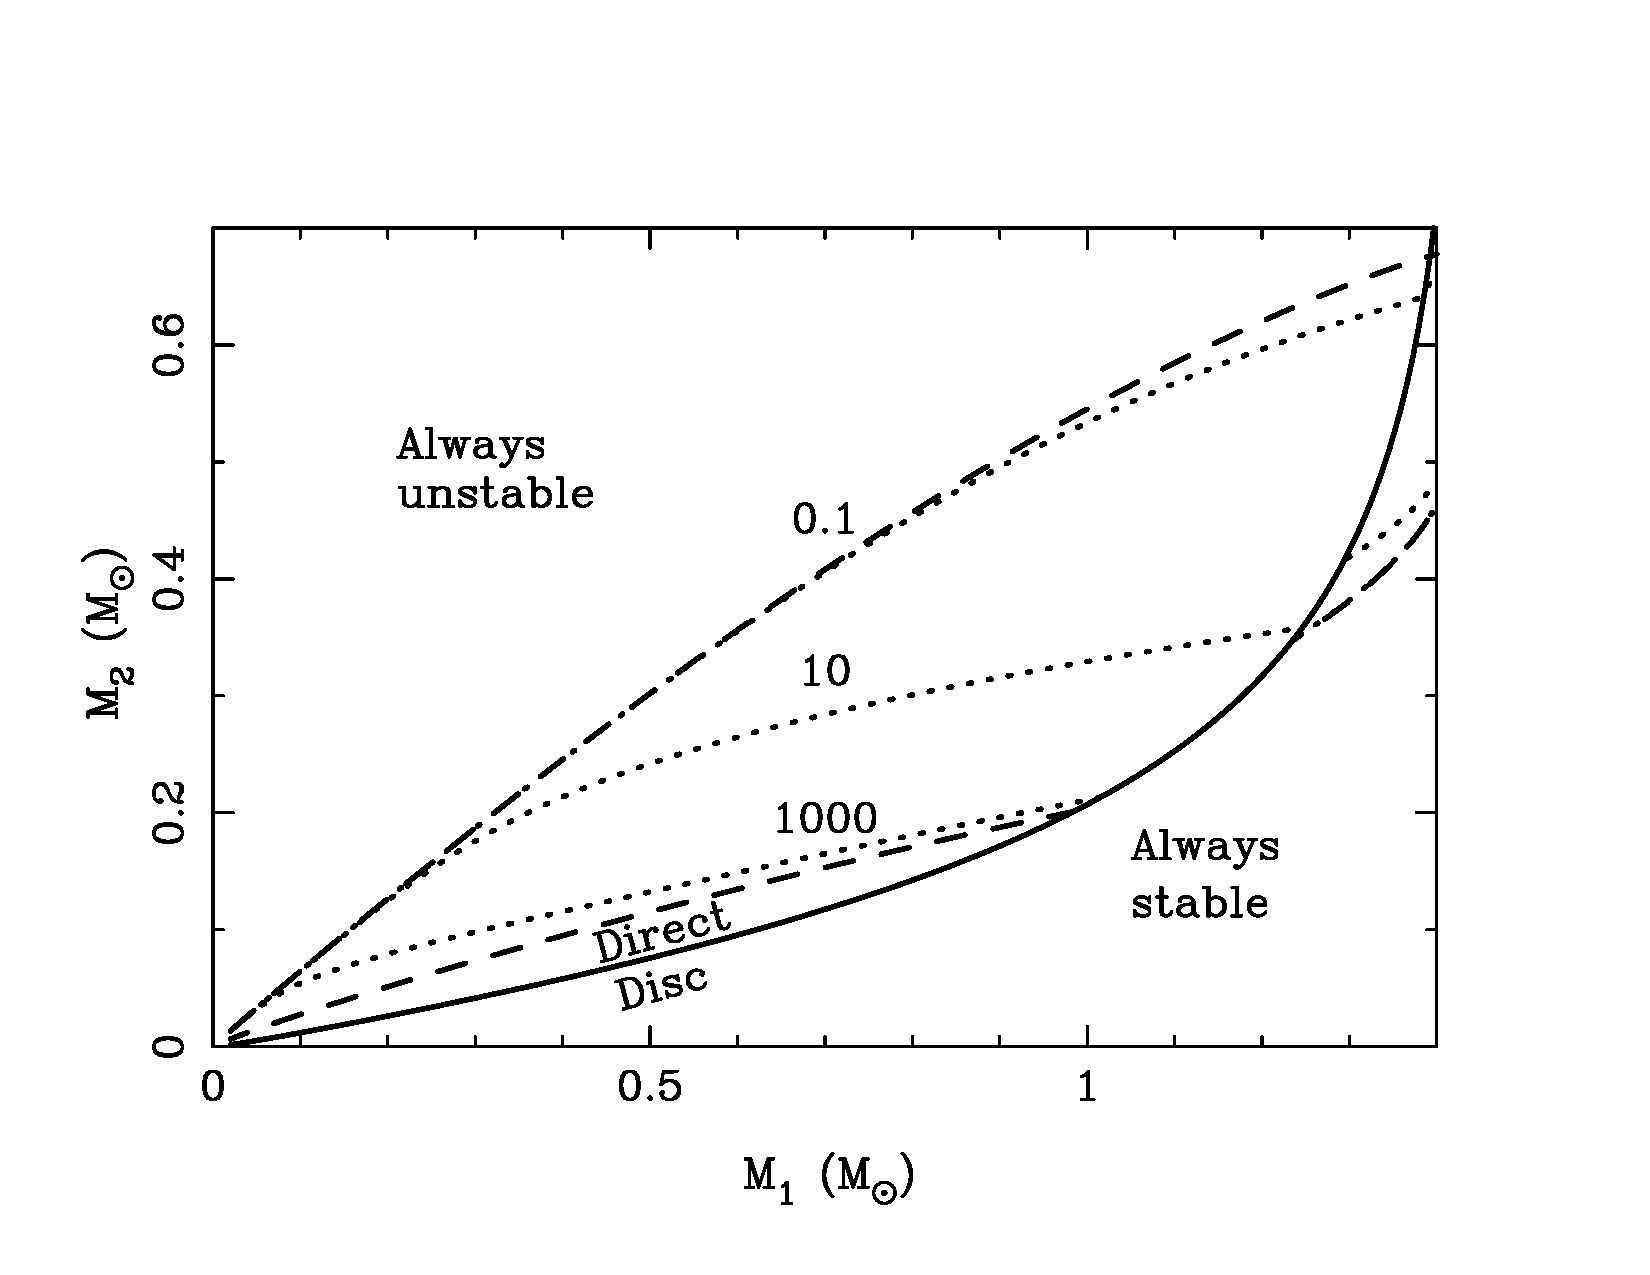
\includegraphics[angle=0,width=0.65\columnwidth]{introduction/figures/marsns04_stab.pdf}
\caption{Regions of stable and unstable mass transfer for the WD merger parameter space from \citeauthor{marsns04} (\citeyear{marsns04}; their Fig. 1).  $M_1$ is \Ma\, and $M_2$ is \Md.  The upper dashed line is a more accurate estimate for Eqn. \ref{eq:c1_qcrit} (that accounts for the accretor's moment of inertia), and the lower dashed one that for Eqn. \ref{eq:c1_qcrit2}.  The solid ``Direct/Disc'' line represents the transition between direct impact and disk accretion.  Dotted lines represent the boundary between stable and unstable mass transfer when the tidal synchronization timescale $\tau_\mrm{s}$ is $1000$, $10$ and $0.1\,\mrm{yr}$.}
\label{fig:c1_stability}
\end{figure}

The question then becomes which stability criterion better represents mass transfer in WD binaries.  In the absence of other sources of spin-orbit coupling, this is determined solely by whether disk or direct impact accretion occurs.  Following \cite{lubos75}, \cite{nele+01} determines when one transitions into the other by calculating the point where the minimum radius reached by the accretion stream becomes larger than the accretor; the corresponding critical surface in the merger mass parameter space is plotted in Fig. \ref{fig:c1_stability}.  For $0.4 \leq \Ma \leq 1.0$, the line falls around $\qm = 0.15$, below even Eqn. \ref{eq:c1_qcrit3}.

Tides within the WDs can substitute for disks for spin-orbit coupling.  While traditional estimates of the spin-orbit synchronization timescale in WD binaries ranges from $\tau_{S} \sim 10^{12}$ yr for radiative damping to $\tau_{S} \sim 10^{15}$ yr for molecular viscosity \citep{marsns04}, other sources of dissipation, such as turbulent viscosity \citep{mochl89}, may lead to much shorter $\tau_{S}$.  Recent work \citep{fulll12, burk+13, fulll14} show resonant coupling between tidal forces and stellar pulsations favor a much shorter $\tau_\mrm{s}$ (though exactly how short remains unclear; \citealt{fulll14}).  Semi-analytical calculations \citep{marsns04,gokhpf07, kremsk15}, however, suggest that even for $\tau_\mrm{s}$ as small as $10\,\mrm{yr}$, all the systems we consider in this thesis should still experience unstable mass transfer and merge.  All these systems also merge in simulations that more accurately model the binary at the onset of mass transfer \citep{dan+11, dan+12}, and so we proceed under the notion that all our binaries should merge.  We note that there is evidence \citep{shen15, brow+16} that even He - CO WD binaries with extremely low $\qm$ do so as well.

% THESIS NOTE: While recent merger simulations have favored synchronized initial conditions (rask+12, 14, dan+12, 14), whether or not tides can sychronize WD binaries remains an open question (dan+14, 2016ApJ...821...67S).  Moreover, dan+14 find that during the merger itself, neither WD is able to maintain its spin against its orbital period as the WD separation reduces dramatically over only a few binary orbits.

%Estimates of the synchronization timescale in binary systems give $\tau_{S} \sim 10^{12}$ yr from radiative damping, and $\tau_{S} \sim 10^{15}$ yr from viscosity \citep{marsns04}.  To compare, the timescale for angular momentum loss from gravitational wave radiation is \citep{segrcm97}

%\noindent In the latter stages of evolution, this value is around $\tau_{S} \sim 10^{6}$ yr.  It is then likely that neither donor nor accretor are synchronized at the time of merger\footnote{A close-in WD binary should merger within $10^8$ to $10^9$ yrs after formation \cite{segrcm97}.  Of course, any transients caused by mergers seen today must have occured within this time!}.  Turbulent viscosity and non-radial mode excitation, on the other hand, can potentially have $\tau_{S} << 500$ yr, and even small magnetic fields, properly oriented, can significantly enhance viscosity \citep{marsns04,ibentf98}.  Also, the viscous timescale scales as $a^6$, while Eqn. \ref{gravtimescale} scales as $a^4$; this indicates that should viscosity ever synchronize a WD binary, this binary will be synchronized for the remainder of its inspiral \citep{ibentf98}.  Whether or not a binary will be synchronized is still largely an unsolved problem \citep{mars11}.

%If we were to suppose a WD system could synchronize, then viscous dissipation should heat up both WDs significantly.  \cite{ibentf98} perform long equal-mass binary evolution calculations that assumes the binary system is synchronized, and the rate of tidal heating is equal to the rate of spin kinetic energy increase. (SO DOES IT SAP ROTATION????)  They find that over the course of the last $10^4$ yrs before merger heating from synchronization can increase the temperature of a 1.0 {\Msun} (with a 1.0 {\Msun} companion) by an order of magnitude.  While most of the thermal energy that is radiated away during this heat-up is in the form of neutrinos, the EM luminosity increases by almost five orders of magnitude.  At the time of merger, each 1.0 {\Msun} WD would shine with $\sim 100$ L$_{\odot}$ and have a temperature of $\sim 10^8$ K, making the system a significant X-ray source.  The luminosity just before merger increases with WD mass, and the period of time over which luminosity increase occurs drops with WD mass: a 0.3 {\Msun} with an equal-mass companion will increase in luminosity by two orders of magnitude over $10^6$ yr.  If the efficiency by which rotational energy is converted to thermal energy is reduced to 10\% the maximum efficiency in the 1.0-1.0 {\Msun} binary, the final luminosity drops by a factor of about 1000.  In all cases simulated, \citeauthor{ibentf98} found temperatures were insufficient to ignite nuclear fusion.  The periods of increased luminosity are all in the range of $10^2 - 10^6$ years, which, while short compared to the liftime of the binary, are far too long to be considered transients.


